\section{sequence}

\begin{flushleft}
Afin de compléter mon extension, j'ai introduit deux diagrammes de séquences, un premier nommé \textbf{Comparer les données de consommations} et un deuxième nommé \textbf{Gérer les données} qui est le même que celui de la base à quelques différences près.
\end{flushleft}

\begin{flushleft}
Dans le cas du premier, nous retrouvons un cas de base. c'est-à-dire que le client n'a qu'à appeler la méthode \textbf{getConsumptionOfSimulation}, le token est vérifié et si ce dernier est correct alors, dans ce cas, nous appelons \textbf{getConsumptionOfSimulation} dans la classe \textbf{ClientDB}.
\end{flushleft}

\begin{figure}[h]
\centering
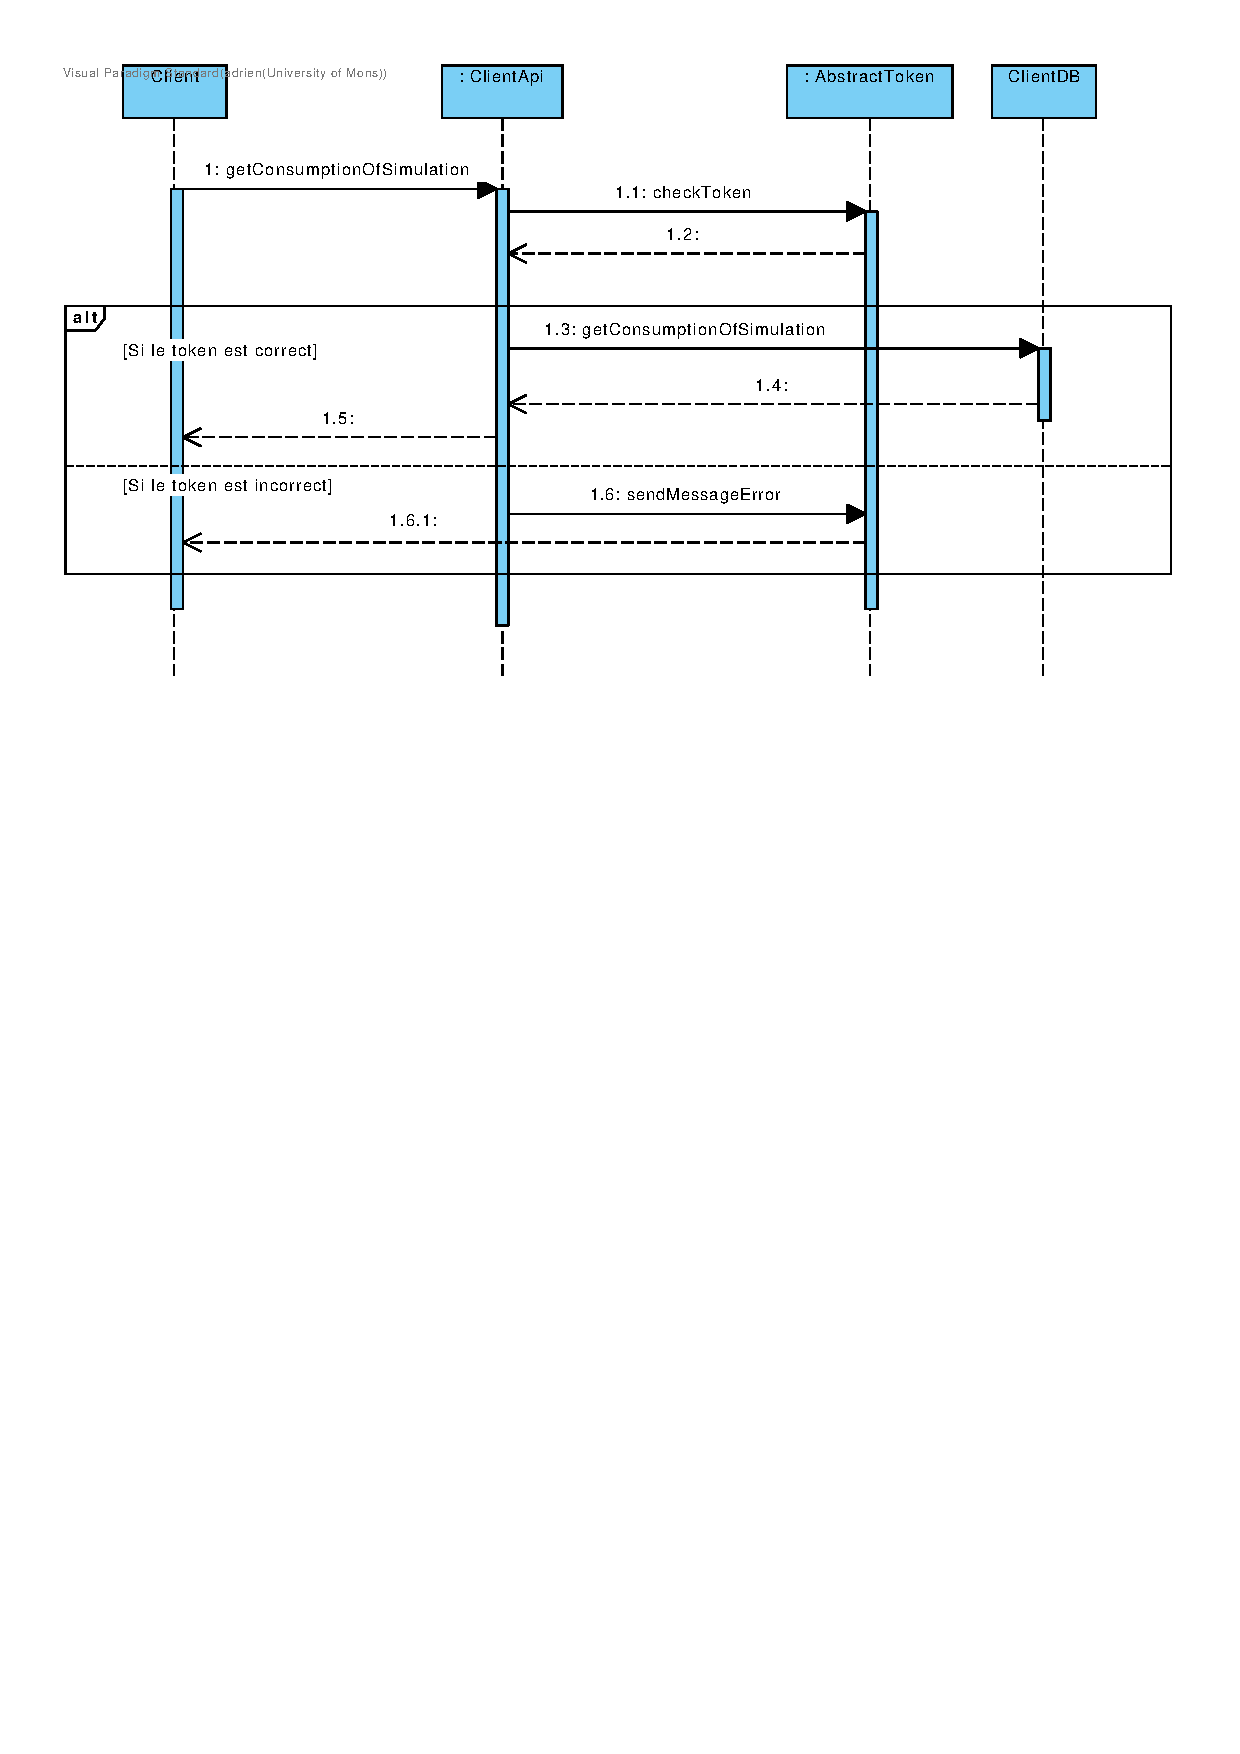
\includegraphics[width=1.3\textwidth]{extension-adrien/Sequence/img/Comparer.pdf}
\end{figure}

\begin{flushleft}
Dans le deuxième cas, que ça soit pour ajouter des données ou les changer, nous vérifions dans la classe \textbf{CommonDB} que la donnée est normale grâce à \textbf{isNormalData}. Si cette donnée est anormale, nous appelons la méthode statique \textbf{sendEmail} de la classe \textbf{App} pour envoyer un mail d'information.
\end{flushleft}

\begin{figure}[h]
\centering
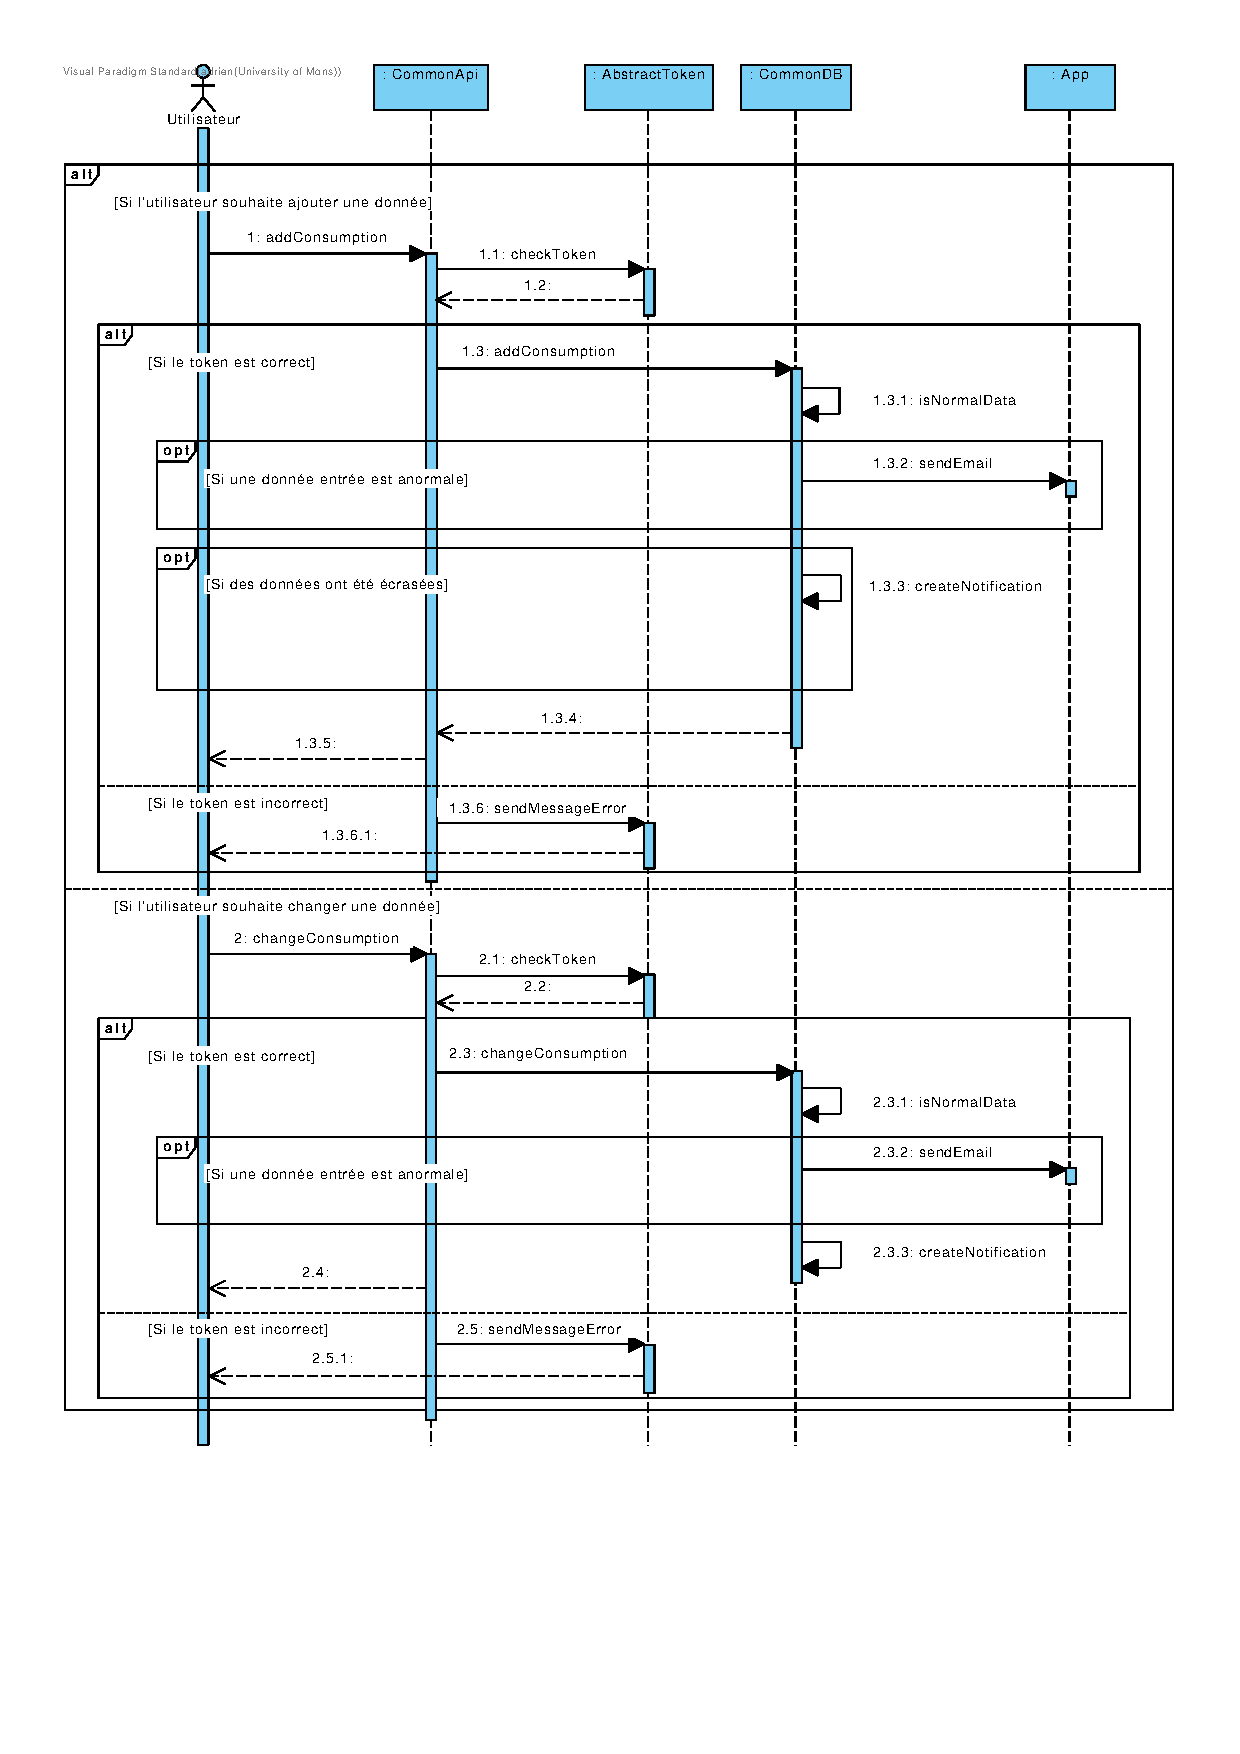
\includegraphics[width=1.3\textwidth]{extension-adrien/Sequence/img/Gerer.pdf}
\end{figure}
